% options for packages loaded elsewhere
\PassOptionsToPackage{unicode=true}{hyperref}
\PassOptionsToPackage{hyphens}{url}

% specify apa6 document mode with command to have a default
\newcommand{\pandocDocMode}{man}

% apa6 mode and class options
\documentclass[\pandocDocMode,longtable, floatsintext, noextraspace]{apa6}
% \documentclass[
%   %     \pandocDocMode,longtable
%   %   
% ]{apa6}

% for mode selection options
\usepackage{ifthen}

\newcommand{\forceLongTablePkg}{}

% % setup mode ifs
% \newif\ifmanmode
% \newif\ifdocmode
% \newif\ifjoumode
% \ifthenelse{\equal{\string \pandocDocMode}{\string man}}{
%     \manmodetrue
% }{
%     \renewcommand{\forceLongTablePkg}{longtable}
%     \ifthenelse{\equal{\string \pandocDocMode}{\string doc}}{
%         \docmodetrue
%     }{
%         \ifthenelse{\equal{\string \pandocDocMode}{\string jou}}{
%             \joumodetrue
%         }{
% % None
% }}}


\usepackage{\forceLongTablePkg}

% % % man mode uses the endfloat package,
% % this will try to set tables and figures at the end for longtables too
% \ifmanmode
% \DeclareDelayedFloatFlavor{longtable}{table}
% \fi
% 
% other packages
\usepackage{lmodern}
\usepackage{amsmath,amssymb}
\usepackage{ifxetex,ifluatex}
\usepackage{fixltx2e} % provides \textsubscript

% handle different types of tex engines
% if pdftex
\ifnum 0\ifxetex 1\fi\ifluatex 1\fi=0
  \usepackage[T1]{fontenc}
  \usepackage[utf8]{inputenc}
  \usepackage{textcomp} % provides euro and other symbols
% if luatex or xelatex
\else
  \usepackage{unicode-math}
  \defaultfontfeatures{Ligatures=TeX,Scale=MatchLowercase}
\fi

% other language options
\usepackage[american]{babel}
\usepackage{csquotes}
\usepackage{microtype}

% disable microtype protrusion for tt fonts
\UseMicrotypeSet[protrusion]{basicmath}

\usepackage{graphicx,grffile}
% Scale images if necessary, so that they will not overflow the page
% margins by default, and it is still possible to overwrite the defaults
% using explicit options in \includegraphics[width, height, ...]{}
\makeatletter
\def\maxwidth{\ifdim\Gin@nat@width>\linewidth\linewidth\else\Gin@nat@width\fi}
\def\maxheight{\ifdim\Gin@nat@height>\textheight\textheight\else\Gin@nat@height\fi}
\makeatother
\setkeys{Gin}{width=\maxwidth,height=\maxheight,keepaspectratio}

\usepackage{booktabs}
\usepackage{caption}
\usepackage{subcaption}

% Pandoc stuff
\let\tightlist\relax % empty pandoc tight list command

% Hyperlinks and other metadata in pdf
\usepackage{hyperref}
\hypersetup{
            pdftitle={Exception Handling and File Processing},
            pdfauthor={Thomas Culpepper},
            colorlinks=false,
            linkcolor=Black,
            citecolor=Black,
            urlcolor=Black,
            pdfborder={0 0 0},
            breaklinks=true}
\urlstyle{same} % don't use monospace font for urls



\usepackage{color}
\usepackage{fancyvrb}
\newcommand{\VerbBar}{|}
\newcommand{\VERB}{\Verb[commandchars=\\\{\}]}
\DefineVerbatimEnvironment{Highlighting}{Verbatim}{commandchars=\\\{\}}
% Add ',fontsize=\small' for more characters per line
\newenvironment{Shaded}{}{}
\newcommand{\AlertTok}[1]{\textcolor[rgb]{1.00,0.00,0.00}{\textbf{#1}}}
\newcommand{\AnnotationTok}[1]{\textcolor[rgb]{0.38,0.63,0.69}{\textbf{\textit{#1}}}}
\newcommand{\AttributeTok}[1]{\textcolor[rgb]{0.49,0.56,0.16}{#1}}
\newcommand{\BaseNTok}[1]{\textcolor[rgb]{0.25,0.63,0.44}{#1}}
\newcommand{\BuiltInTok}[1]{#1}
\newcommand{\CharTok}[1]{\textcolor[rgb]{0.25,0.44,0.63}{#1}}
\newcommand{\CommentTok}[1]{\textcolor[rgb]{0.38,0.63,0.69}{\textit{#1}}}
\newcommand{\CommentVarTok}[1]{\textcolor[rgb]{0.38,0.63,0.69}{\textbf{\textit{#1}}}}
\newcommand{\ConstantTok}[1]{\textcolor[rgb]{0.53,0.00,0.00}{#1}}
\newcommand{\ControlFlowTok}[1]{\textcolor[rgb]{0.00,0.44,0.13}{\textbf{#1}}}
\newcommand{\DataTypeTok}[1]{\textcolor[rgb]{0.56,0.13,0.00}{#1}}
\newcommand{\DecValTok}[1]{\textcolor[rgb]{0.25,0.63,0.44}{#1}}
\newcommand{\DocumentationTok}[1]{\textcolor[rgb]{0.73,0.13,0.13}{\textit{#1}}}
\newcommand{\ErrorTok}[1]{\textcolor[rgb]{1.00,0.00,0.00}{\textbf{#1}}}
\newcommand{\ExtensionTok}[1]{#1}
\newcommand{\FloatTok}[1]{\textcolor[rgb]{0.25,0.63,0.44}{#1}}
\newcommand{\FunctionTok}[1]{\textcolor[rgb]{0.02,0.16,0.49}{#1}}
\newcommand{\ImportTok}[1]{#1}
\newcommand{\InformationTok}[1]{\textcolor[rgb]{0.38,0.63,0.69}{\textbf{\textit{#1}}}}
\newcommand{\KeywordTok}[1]{\textcolor[rgb]{0.00,0.44,0.13}{\textbf{#1}}}
\newcommand{\NormalTok}[1]{#1}
\newcommand{\OperatorTok}[1]{\textcolor[rgb]{0.40,0.40,0.40}{#1}}
\newcommand{\OtherTok}[1]{\textcolor[rgb]{0.00,0.44,0.13}{#1}}
\newcommand{\PreprocessorTok}[1]{\textcolor[rgb]{0.74,0.48,0.00}{#1}}
\newcommand{\RegionMarkerTok}[1]{#1}
\newcommand{\SpecialCharTok}[1]{\textcolor[rgb]{0.25,0.44,0.63}{#1}}
\newcommand{\SpecialStringTok}[1]{\textcolor[rgb]{0.73,0.40,0.53}{#1}}
\newcommand{\StringTok}[1]{\textcolor[rgb]{0.25,0.44,0.63}{#1}}
\newcommand{\VariableTok}[1]{\textcolor[rgb]{0.10,0.09,0.49}{#1}}
\newcommand{\VerbatimStringTok}[1]{\textcolor[rgb]{0.25,0.44,0.63}{#1}}
\newcommand{\WarningTok}[1]{\textcolor[rgb]{0.38,0.63,0.69}{\textbf{\textit{#1}}}}



% Title page stuff
\title{Exception Handling and File Processing}
\shorttitle{Exception Handling and File Processing}
\author{Thomas Culpepper}
\affiliation{CSC310 Module 1 Case\\Trident University International}


% 
% 
% 

% \newcommand{\journalOptions}{
% \ifthenelse{\equal{\string \pandocDocMode}{\string jou}}{

% % Journal specific commands may go here:
% % % % % % }{}
% }

% \journalOptions{}


% table caption width
\makeatletter
\newcommand\LastLTentrywidth{1em}
\newlength\longtablewidth
\setlength{\longtablewidth}{1in}
\newcommand\getlongtablewidth{%
\begingroup
\ifcsname LT@\roman{LT@tables}\endcsname
\global\longtablewidth=0pt
\renewcommand\LT@entry[2]{\global\advance\longtablewidth by ##2\relax\gdef\LastLTentrywidth{##2}}%
\@nameuse{LT@\roman{LT@tables}}%
\fi
\endgroup}


%% pandoc-tablenos: environment to disable table caption prefixes
\makeatletter
\newcounter{tableno}
\newenvironment{tablenos:no-prefix-table-caption}{
  \caption@ifcompatibility{}{
    \let\oldthetable\thetable
    \let\oldtheHtable\theHtable
    \renewcommand{\thetable}{tableno:\thetableno}
    \renewcommand{\theHtable}{tableno:\thetableno}
    \stepcounter{tableno}
    \captionsetup{labelformat=empty}
  }
}{
  \caption@ifcompatibility{}{
    \captionsetup{labelformat=default}
    \let\thetable\oldthetable
    \let\theHtable\oldtheHtable
    \addtocounter{table}{-1}
  }
}
\makeatother


% PREAMBLE END
% --------------
% DOCUMENT START

\begin{document}
\maketitle

Lorem ipsum dolor sit amet, consectetur adipiscing elit. Nullam in
tellus ornare libero elementum bibendum a sit amet magna. Vestibulum eu
ex vitae odio hendrerit hendrerit. Integer aliquet, nisi non hendrerit
porta, dui eros laoreet velit, sit amet finibus justo risus sit amet
tortor. Mauris at sapien libero. Vestibulum eleifend purus quis elit
pulvinar fermentum id id massa. Proin tincidunt nisi a vehicula rhoncus.
Nullam ornare pretium accumsan. Pellentesque sollicitudin augue lorem,
sit amet vulputate nunc dictum sed. Maecenas in feugiat felis, et
facilisis enim. Etiam interdum, elit sit amet interdum commodo, dolor
eros suscipit orci, vitae porta massa nunc nec odio. Vivamus quis arcu
erat. Sed lorem lacus, scelerisque quis facilisis ac, volutpat vitae
ante. Nulla tellus mi, aliquet ut laoreet ut, lobortis cursus nunc. In
et facilisis mi, sodales finibus mauris. Cras a nisi suscipit quam
accumsan dapibus in sed tortor. Sed gravida nibh justo, eu mattis lectus
semper ornare.

Quisque viverra ex vitae lorem dictum, at facilisis odio tempus. Proin
libero risus, gravida et bibendum eget, ornare sit amet mi. Phasellus
vitae suscipit augue. Etiam iaculis mauris in suscipit interdum. Sed at
nisl dolor. Ut ut sollicitudin tortor, eget porttitor erat. Vestibulum
viverra ac nibh sit amet pretium. Ut commodo scelerisque neque tempor
eleifend. Nulla facilisi. In mollis est quis urna efficitur, id porta
leo maximus. Ut vel augue enim. Aliquam non odio pharetra lorem gravida
facilisis.

\hypertarget{mycode}{%
\label{mycode}}%
\begin{Shaded}
\begin{Highlighting}[numbers=left,,firstnumber=100,]
\KeywordTok{import} \ImportTok{javax}\OperatorTok{.}\ImportTok{swing}\OperatorTok{.}\ImportTok{JOptionPane}\OperatorTok{;}
\KeywordTok{import} \ImportTok{java}\OperatorTok{.}\ImportTok{util}\OperatorTok{.}\ImportTok{regex}\OperatorTok{.*;}

\KeywordTok{public} \KeywordTok{class}\NormalTok{ CalcTaxes }\OperatorTok{\{}
    \KeywordTok{public} \DataTypeTok{static} \DataTypeTok{void} \FunctionTok{main}\OperatorTok{(}\BuiltInTok{String}\OperatorTok{[]}\NormalTok{ args}\OperatorTok{)} \OperatorTok{\{}
        \DataTypeTok{boolean}\NormalTok{ calcAgain }\OperatorTok{=} \KeywordTok{true}\OperatorTok{;} \CommentTok{//control to run again or exit}

        \BuiltInTok{JOptionPane}\OperatorTok{.}\FunctionTok{showMessageDialog}\OperatorTok{(}
            \KeywordTok{null}\OperatorTok{,} \StringTok{"This program will calculate your federal and state taxes"}\OperatorTok{);}

        \ControlFlowTok{while} \OperatorTok{(}\NormalTok{calcAgain}\OperatorTok{)} \OperatorTok{\{}
            \BuiltInTok{String}\NormalTok{ validationPattern }\OperatorTok{=} \KeywordTok{null}\OperatorTok{;}
            \BuiltInTok{String}\NormalTok{ errorMessage }\OperatorTok{=} \KeywordTok{null}\OperatorTok{;}
            \BuiltInTok{String} \OperatorTok{[]}\NormalTok{ userInputs }\OperatorTok{=} \KeywordTok{new} \BuiltInTok{String}\OperatorTok{[}\DecValTok{4}\OperatorTok{];} \CommentTok{//array to hold user input strings}
            \BuiltInTok{String} \OperatorTok{[][]}\NormalTok{ inputRequests }\OperatorTok{=} \OperatorTok{\{} \CommentTok{//input requests and expected type (num or str)}
                \OperatorTok{\{}\StringTok{"Please enter your name:"}\OperatorTok{,}\StringTok{"str"}\OperatorTok{\},}
                \OperatorTok{\{}\StringTok{"Enter your yearly income"}\OperatorTok{,}\StringTok{"num"}\OperatorTok{\},}
                \OperatorTok{\{}\StringTok{"Enter your Federal tax rate (\%):"}\OperatorTok{,}\StringTok{"num"}\OperatorTok{\},}
                \OperatorTok{\{}\StringTok{"Enter your State tax rate (\%):"}\OperatorTok{,}\StringTok{"num"}\OperatorTok{\}}
            \OperatorTok{\};}
\end{Highlighting}
\end{Shaded}

Donec dui nunc, convallis nec lectus non, accumsan dictum lorem. Nam
viverra, libero sed pulvinar tincidunt, mi augue rhoncus neque, et
venenatis turpis velit quis odio. Nulla feugiat vitae urna id congue.
Pellentesque efficitur facilisis hendrerit. Quisque vehicula vel risus
vel faucibus. Quisque eleifend mattis maximus. Interdum et malesuada
fames ac ante ipsum primis in faucibus.

Mauris blandit nisi non dapibus lobortis. Morbi sit amet elementum
libero, sed laoreet est. Sed auctor nibh ac semper faucibus. Fusce
pretium ultrices neque, sit amet luctus mi sollicitudin vel. Suspendisse
efficitur metus quis dui posuere, id vehicula dui pulvinar. Donec sit
amet dapibus diam. Donec libero sem, fringilla et cursus ut, lacinia
quis nisl. Donec ullamcorper malesuada purus tempor venenatis. Morbi vel
ante vulputate, feugiat velit at, pellentesque odio. Phasellus nec justo
aliquet, maximus quam a, venenatis ligula. Ut porttitor metus id diam
sollicitudin, non lacinia augue faucibus.

Morbi quis lobortis neque. Aenean blandit, dui et sollicitudin
ullamcorper, neque leo rhoncus libero, vitae ullamcorper ex massa vitae
dolor. Nam placerat posuere nulla ac consectetur. In porta ornare nisi
quis suscipit. Quisque sed turpis sit amet mi sagittis molestie ac in
nisi. Integer ligula nulla, lobortis ac elementum sit amet, ultricies
eget leo. Nulla ullamcorper dolor vel neque pretium, quis porttitor est
consequat. Donec euismod mauris sit amet dui fermentum, eget tempor dui
suscipit. Ut eros risus, semper in sollicitudin vel, lacinia a sapien.
Duis fermentum mauris nec diam vestibulum fringilla.

\hypertarget{mycodemore}{%
\label{mycodemore}}%
\begin{Shaded}
\begin{Highlighting}[numbers=left,,firstnumber=100,]
            \ControlFlowTok{for} \OperatorTok{(}\DataTypeTok{int}\NormalTok{ i}\OperatorTok{=}\DecValTok{0}\OperatorTok{;}\NormalTok{ i }\OperatorTok{\textless{}}\NormalTok{ inputRequests}\OperatorTok{.}\FunctionTok{length}\OperatorTok{;}\NormalTok{ i}\OperatorTok{++)} \OperatorTok{\{}
\NormalTok{                userInputs}\OperatorTok{[}\NormalTok{i}\OperatorTok{]} \OperatorTok{=} \BuiltInTok{JOptionPane}\OperatorTok{.}\FunctionTok{showInputDialog}\OperatorTok{(}\NormalTok{inputRequests}\OperatorTok{[}\NormalTok{i}\OperatorTok{][}\DecValTok{0}\OperatorTok{]);}
                \ControlFlowTok{if} \OperatorTok{(}\NormalTok{userInputs}\OperatorTok{[}\NormalTok{i}\OperatorTok{]} \OperatorTok{==} \KeywordTok{null}\OperatorTok{)} \OperatorTok{\{} \CommentTok{// Exit cleanly if user hits cancel}
                    \BuiltInTok{System}\OperatorTok{.}\FunctionTok{exit}\OperatorTok{(}\DecValTok{0}\OperatorTok{);}
                \OperatorTok{\}}
                \ControlFlowTok{else} \ControlFlowTok{if} \OperatorTok{(}\NormalTok{inputRequests}\OperatorTok{[}\NormalTok{i}\OperatorTok{][}\DecValTok{1}\OperatorTok{].}\FunctionTok{equals}\OperatorTok{(}\StringTok{"num"}\OperatorTok{))\{}
\NormalTok{                    validationPattern }\OperatorTok{=} \StringTok{"\^{}}\SpecialCharTok{\textbackslash{}\textbackslash{}}\StringTok{d+$|\^{}{-}?}\SpecialCharTok{\textbackslash{}\textbackslash{}}\StringTok{d*}\SpecialCharTok{\textbackslash{}\textbackslash{}}\StringTok{.}\SpecialCharTok{\textbackslash{}\textbackslash{}}\StringTok{d\{2\}$"}\OperatorTok{;} \CommentTok{// match integer or 2 place decimal}
\NormalTok{                    errorMessage }\OperatorTok{=} \StringTok{"Please enter a number }\SpecialCharTok{\textbackslash{}n}\StringTok{(000 or 00.00)"}\OperatorTok{;}
                \OperatorTok{\}}
                \ControlFlowTok{else} \ControlFlowTok{if} \OperatorTok{(}\NormalTok{inputRequests}\OperatorTok{[}\NormalTok{i}\OperatorTok{][}\DecValTok{1}\OperatorTok{].}\FunctionTok{equals}\OperatorTok{(}\StringTok{"str"}\OperatorTok{))} \OperatorTok{\{}
\NormalTok{                    validationPattern }\OperatorTok{=} \StringTok{"\^{}[A{-}Za{-}z]+}\SpecialCharTok{\textbackslash{}\textbackslash{}}\StringTok{s*[A{-}Za{-}z]*$"}\OperatorTok{;} \CommentTok{// match name and optional 2nd name}
\NormalTok{                    errorMessage }\OperatorTok{=} \StringTok{"Try again./nNo numbers or symbols please"}\OperatorTok{;}
                \OperatorTok{\}}
                \ControlFlowTok{else} \OperatorTok{\{}
                    \BuiltInTok{JOptionPane}\OperatorTok{.}\FunctionTok{showMessageDialog}\OperatorTok{(}
                        \KeywordTok{null}\OperatorTok{,} \StringTok{"Illegal Input type Option. Please contact the developer."}\OperatorTok{);}
                    \ControlFlowTok{throw} \KeywordTok{new} \BuiltInTok{IllegalArgumentException}\OperatorTok{(}
                        \StringTok{"Input type option invalid. Only \textquotesingle{}num\textquotesingle{} or \textquotesingle{}str\textquotesingle{} allowed"}\OperatorTok{);}
                \OperatorTok{\}}

                \BuiltInTok{Pattern}\NormalTok{ p }\OperatorTok{=} \BuiltInTok{Pattern}\OperatorTok{.}\FunctionTok{compile}\OperatorTok{(}\NormalTok{validationPattern}\OperatorTok{);}
                \BuiltInTok{Matcher}\NormalTok{ m }\OperatorTok{=}\NormalTok{ p}\OperatorTok{.}\FunctionTok{matcher}\OperatorTok{(}\NormalTok{userInputs}\OperatorTok{[}\NormalTok{i}\OperatorTok{]);}
                \ControlFlowTok{if} \OperatorTok{(!}\NormalTok{m}\OperatorTok{.}\FunctionTok{find}\OperatorTok{())\{} 
                    \BuiltInTok{JOptionPane}\OperatorTok{.}\FunctionTok{showMessageDialog}\OperatorTok{(}\KeywordTok{null}\OperatorTok{,}\NormalTok{ errorMessage}\OperatorTok{);}
\NormalTok{                    i}\OperatorTok{{-}{-};}
                \OperatorTok{\}}
            \OperatorTok{\}}

            \DataTypeTok{double}\NormalTok{ yearlyIncome }\OperatorTok{=} \BuiltInTok{Double}\OperatorTok{.}\FunctionTok{parseDouble}\OperatorTok{(}\NormalTok{userInputs}\OperatorTok{[}\DecValTok{1}\OperatorTok{]);}
            \DataTypeTok{double}\NormalTok{ fedTaxRate }\OperatorTok{=} \BuiltInTok{Double}\OperatorTok{.}\FunctionTok{parseDouble}\OperatorTok{(}\NormalTok{userInputs}\OperatorTok{[}\DecValTok{2}\OperatorTok{])} \OperatorTok{/} \DecValTok{100}\OperatorTok{;}
            \DataTypeTok{double}\NormalTok{ stateTaxRate }\OperatorTok{=} \BuiltInTok{Double}\OperatorTok{.}\FunctionTok{parseDouble}\OperatorTok{(}\NormalTok{userInputs}\OperatorTok{[}\DecValTok{3}\OperatorTok{])} \OperatorTok{/} \DecValTok{100}\OperatorTok{;}
            \DataTypeTok{double}\NormalTok{ fedTaxDue }\OperatorTok{=}\NormalTok{ yearlyIncome }\OperatorTok{*}\NormalTok{ fedTaxRate}\OperatorTok{;}
            \DataTypeTok{double}\NormalTok{ stateTaxDue }\OperatorTok{=}\NormalTok{ yearlyIncome }\OperatorTok{*}\NormalTok{ stateTaxRate}\OperatorTok{;}

            \BuiltInTok{JOptionPane}\OperatorTok{.}\FunctionTok{showMessageDialog}\OperatorTok{(}\KeywordTok{null}\OperatorTok{,}\NormalTok{ userInputs}\OperatorTok{[}\DecValTok{0}\OperatorTok{]} \OperatorTok{+} \StringTok{"}\SpecialCharTok{\textbackslash{}n}\StringTok{Your Federal Taxes are: $"} 
                \OperatorTok{+}\NormalTok{ fedTaxDue }\OperatorTok{+} \StringTok{"}\SpecialCharTok{\textbackslash{}n}\StringTok{Your State taxes are: $"} \OperatorTok{+}\NormalTok{ stateTaxDue}\OperatorTok{);}

            \DataTypeTok{int}\NormalTok{ reply }\OperatorTok{=} \BuiltInTok{JOptionPane}\OperatorTok{.}\FunctionTok{showConfirmDialog}\OperatorTok{(}\KeywordTok{null}\OperatorTok{,} \StringTok{"Would you like to calculate more?"}\OperatorTok{,} 
                \StringTok{"Run Again?"}\OperatorTok{,}  \BuiltInTok{JOptionPane}\OperatorTok{.}\FunctionTok{YES\_NO\_OPTION}\OperatorTok{);}
            \ControlFlowTok{if} \OperatorTok{(}\NormalTok{reply }\OperatorTok{==} \BuiltInTok{JOptionPane}\OperatorTok{.}\FunctionTok{NO\_OPTION}\OperatorTok{)} \OperatorTok{\{}
\NormalTok{                    calcAgain }\OperatorTok{=} \KeywordTok{false}\OperatorTok{;}
            \OperatorTok{\}}
        \OperatorTok{\}}
    \OperatorTok{\}} 
\OperatorTok{\}}
\end{Highlighting}
\end{Shaded}

Lorem ipsum dolor sit amet, consectetur adipiscing elit. Nullam in
tellus ornare libero elementum bibendum a sit amet magna. Vestibulum eu
ex vitae odio hendrerit hendrerit. Integer aliquet, nisi non hendrerit
porta, dui eros laoreet velit, sit amet finibus justo risus sit amet
tortor. Mauris at sapien libero. Vestibulum eleifend purus quis elit
pulvinar fermentum id id massa. Proin tincidunt nisi a vehicula rhoncus.
Nullam ornare pretium accumsan. Pellentesque sollicitudin augue lorem,
sit amet vulputate nunc dictum sed. Maecenas in feugiat felis, et
facilisis enim. Etiam interdum, elit sit amet interdum commodo, dolor
eros suscipit orci, vitae porta massa nunc nec odio. Vivamus quis arcu
erat. Sed lorem lacus, scelerisque quis facilisis ac, volutpat vitae
ante. Nulla tellus mi, aliquet ut laoreet ut, lobortis cursus nunc. In
et facilisis mi, sodales finibus mauris. Cras a nisi suscipit quam
accumsan dapibus in sed tortor. Sed gravida nibh justo, eu mattis lectus
semper ornare.

Quisque viverra ex vitae lorem dictum, at facilisis odio tempus. Proin
libero risus, gravida et bibendum eget, ornare sit amet mi. Phasellus
vitae suscipit augue. Etiam iaculis mauris in suscipit interdum. Sed at
nisl dolor. Ut ut sollicitudin tortor, eget porttitor erat. Vestibulum
viverra ac nibh sit amet pretium. Ut commodo scelerisque neque tempor
eleifend. Nulla facilisi. In mollis est quis urna efficitur, id porta
leo maximus. Ut vel augue enim. Aliquam non odio pharetra lorem gravida
facilisis.

Donec dui nunc, convallis nec lectus non, accumsan dictum lorem. Nam
viverra, libero sed pulvinar tincidunt, mi augue rhoncus neque, et
venenatis turpis velit quis odio. Nulla feugiat vitae urna id congue.
Pellentesque efficitur facilisis hendrerit. Quisque vehicula vel risus
vel faucibus. Quisque eleifend mattis maximus. Interdum et malesuada
fames ac ante ipsum primis in faucibus.

Mauris blandit nisi non dapibus lobortis. Morbi sit amet elementum
libero, sed laoreet est. Sed auctor nibh ac semper faucibus. Fusce
pretium ultrices neque, sit amet luctus mi sollicitudin vel. Suspendisse
efficitur metus quis dui posuere, id vehicula dui pulvinar. Donec sit
amet dapibus diam. Donec libero sem, fringilla et cursus ut, lacinia
quis nisl. Donec ullamcorper malesuada purus tempor venenatis. Morbi vel
ante vulputate, feugiat velit at, pellentesque odio. Phasellus nec justo
aliquet, maximus quam a, venenatis ligula. Ut porttitor metus id diam
sollicitudin, non lacinia augue faucibus.

Morbi quis lobortis neque. Aenean blandit, dui et sollicitudin
ullamcorper, neque leo rhoncus libero, vitae ullamcorper ex massa vitae
dolor. Nam placerat posuere nulla ac consectetur. In porta ornare nisi
quis suscipit. Quisque sed turpis sit amet mi sagittis molestie ac in
nisi. Integer ligula nulla, lobortis ac elementum sit amet, ultricies
eget leo. Nulla ullamcorper dolor vel neque pretium, quis porttitor est
consequat. Donec euismod mauris sit amet dui fermentum, eget tempor dui
suscipit. Ut eros risus, semper in sollicitudin vel, lacinia a sapien.
Duis fermentum mauris nec diam vestibulum fringilla.

\begin{figure}
\hypertarget{fig:screen1}{%
\centering
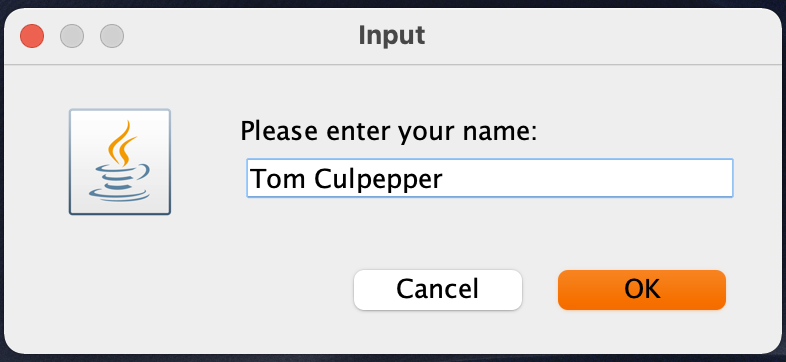
\includegraphics[width=\textwidth,height=1.5in]{media/CSC310-Case1-1.png}
\caption{CalcTaxes Screen 1}\label{fig:screen1}
}
\end{figure}

\hypertarget{references}{%
\subsection{References}\label{references}}





\end{document}